%************************************************
\chapter{Cloud Computing \& The Cloud}\label{ch:infrastructure}
%************************************************
For the past 5 years we have seen the terms "cloud" and "cloud computing" used to describe different services and offers from all around the Internet, but there isn't really a consensus on what the "cloud" really is. So, before we can begin to describe the infrastructure of a Cloud Service, we must first define what the these terms mean and why they are so important to the current IT environment.

\section{Defining the Cloud}
The term "The Cloud" has become a familiar metaphor for the Internet. A lot of people simply refer to everything that is outside of a firewall as "the cloud", but it isn't until you combine the term with the word "computing" that it takes on a different meaning. And with this new meaning come different definitions of what the phrase entitles.\footnote{\url{http://www.infoworld.com/d/cloud-computing/what-cloud-computing-really-means-031}}

For most professionals the term "Cloud Computing" is a synonym for Distributed Computing over a Network. Distributed Computing means the ability to run a computer program on many machines at the same time, thus distributing the working load over all of these machines' processors.\footnote{\url{http://en.wikipedia.org/wiki/Distributed_computing}}

The \ac{NIST} defines Cloud Computing as:
\begin{quotation}
[...] a model for enabling convenient, on-demand network access to a shared pool of configurable computing resources (e.g., networks, servers, storage, applications, and services) that can be rapidly provisioned and released with minimal management effort or service provider interaction.
\footnote{\url{http://www.nist.gov/itl/cloud/upload/cloud-def-v15.pdf}} 
\end{quotation}

This definition makes it clear that Cloud Computing is a model and not a technology, which means there can be many different implementations and variations of the base model, each with its own distinct advantages and disadvantages.

The machines involved in Cloud Computing are usually virtual servers. These virtual servers appear to be, in every sense, real servers, but actually run on a virtual machine that can be scaled up or down depending on the needs of the applications it runs.

So for the purposes of this thesis we will expand on the \ac{NIST} definition of Cloud Computing with the following:
\begin{description}
\item[Cloud:] A distributed network of machines or virtual machines that collaborate within the scope of a given application/service or provide necessary services to said application/service.  
\item[Cloud Computing:] The ability to execute any number of computations on the Cloud, without having to worry about how the data is actually distributed.
\end{description}

Furthermore the term \textsc{Cloud Service} will be given to an application or service that runs on the cloud.

\section{The Infrastructure of the Cloud}

As we described in the previous section, our version of the cloud consists of an array of virtual machines. This array can be hosted on a single physical machine or on several networked machines.

There are many types of virtualization, e. g. Memory, Network, Storage, Hardware and Service Virtualization. The last one encompasses all the previous ones and has been the building block of most of the different Cloud implementations currently available.\footnote{\url{http://www.f5.com/pdf/white-papers/virtualization-defined-wp.pdf}}

It is very interesting that virtualization, the logical abstraction of hardware through a layer of software, has been around, in one way or another, since the mainframe era\cite[p. 3]{williams:2012} and it is now driving a revolution not only in cloud technology and its infrastructure, but also within the Enterprise, allowing businesses to better utilize their IT resources and save money.   

Thanks to the \ac{NIST} definition we also know that cloud computing must be easy to configure, highly accessible, fast to deploy and highly scalable. These are all characteristics of a virtualized system.
\cite{vmware:2007}

There are a few companies that have been pushing the development of virtualization technology, and bringing forth new ideas and improvements to the field. They are \textit{Citrix}, \textit{Microsoft}, \textit{Parallels} and \textit{VMware}.

These companies offer professional virtualization solutions for Enterprises and Individuals looking to build their own cloud infrastructure. Be it on-premises or on a datacenter with rented servers, they offer different products that scale based on the needs of the customer.

A quick look at \autoref{fig:vm} should give you an overview of how virtualization works. 

\begin{figure}[H]
    \begin{center}
        {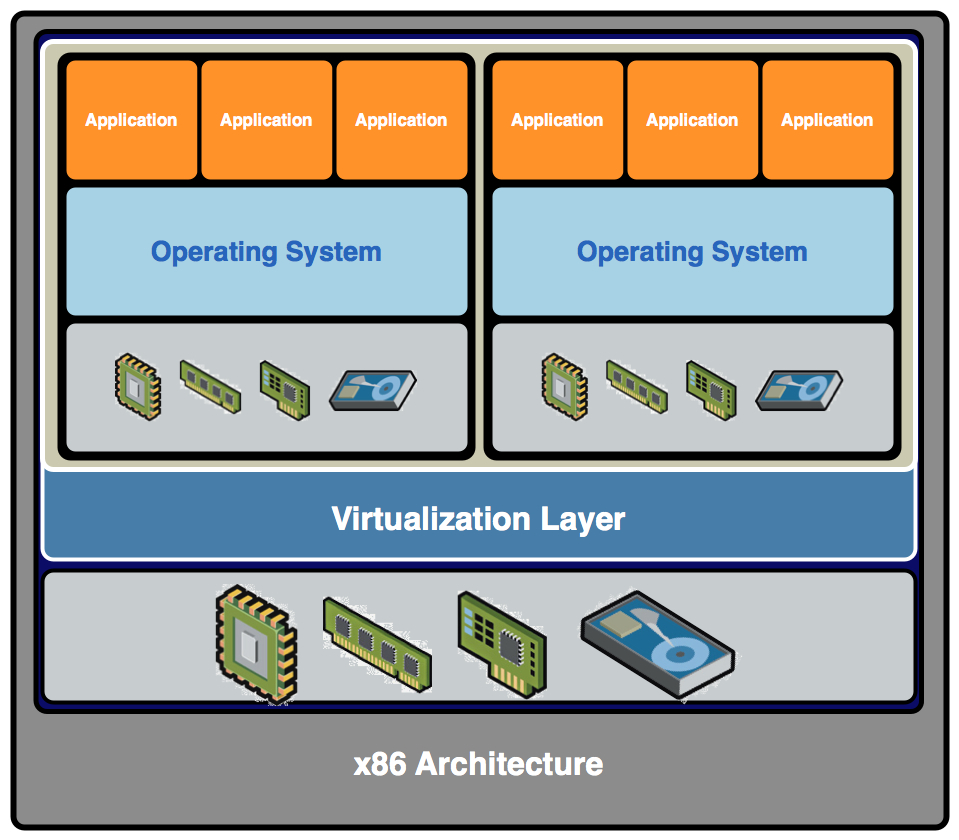
\includegraphics[width=.70\linewidth]{gfx/vm}}
        \caption[Hardware Virtualization]{Hardware Virtualization\footnotemark}\label{fig:vm}
    \end{center}
\end{figure}
\footnotetext{Source: \url{http://www.vmware.com/files/pdf/VMware_paravirtualization.pdf}}\\

Professional Virtualization products are based on one of the three different types of Hardware Virtualization:
\begin{description}
\item[Full Virtualization] uses a combination of direct execution of user requests and binary translation of \ac{OS} requests. It translates kernel code to replace non-virtualizable instructions with new sequences of instructions that have the intended effect on the virtual hardware.

It simplifies migration, portability and scalability of the Guest \ac{OS} and offers the best isolation and security for virtual machines.
\cite[p. 4]{vmware:2007}

\item[Hardware Assisted Virtualization] relies on improvements made by the chip vendors, like Intel and AMD, in order to simplify virtualization techniques.

These improvements target privileged instructions with a new CPU execution mode feature that allows the hypervisor\marginpar{Hypervisor: A software layer in charge of running and managing the virtual machines} to run in a new root mode below the Guest \ac{OS}. Thus, privileged and sensitive calls are automatically trapped by the hypervisor, removing the need for either binary translation or
paravirtualization.
\cite[p. 6]{vmware:2007}

\item[OS Assisted Virtualization/Paravirtualization] It involves modifying the OS kernel to replace non-virtualizable instructions with hypercalls that communicate directly with the virtualization layer hypervisor and its value lies in a smaller overhead.

It is actually easier to modify the Guest \ac{OS} to support Paravirtualization than to build the more sophisticated binary translation support needed for Full Virtualization.
\cite[p. 5]{vmware:2007}
\end{description}


The products of these companies, together with \textsc{QEMU},\marginpar{QEMU is an open source processor emulator and virtualizer that uses full virtualization} provide the infrastructure of most cloud offerings currently available.    

\section{Different Types of Cloud Services}
The breadth of possible applications and services that can run on top of Cloud Technology is astounding, however they can all be classified into three distinct types, \textit{\ac{IaaS}, \ac{PaaS}} and \textit{\ac{SaaS}}. These three types combined are often referred to as \textit{The Cloud Computing Stack} (See \autoref{fig:ipsaas}), but you don't need to be running all of them in order to be using cloud computing.
\cite[p. 8]{mcgrath:2012}  

\begin{description}
\item[Infrastructure as a Service] involves itself with the lowest layer of Cloud Computing, as it provides the components necessary to run any kind of application on top of a physical, or (more often) a virtualized infrastructure.

Providers of \ac{IaaS} usually offer their clients everything they need in order to easily manage and configure their service. This includes the capability to provision processing, storage, networks, and other fundamental computing resources that the customer can use to run any kind of software, including operating systems and applications. 

The provider manages and controls the underlying cloud infrastructure and the user has control over the operating systems, storage and deployed applications.
\cite[p. 8]{sabharwal:2013}

Some examples of \ac{IaaS} Providers include \textit{Amazon}, with its Elastic Cloud service; \textit{ Microsoft}, with Windows Azure; \textit{VMware}, with its vCloud Hybrid service and \textit{DigitalOcean}.
 
\item[Platform as a Service] lays in the middle of the Cloud Computing stack and sits right on top of an already defined infrastructure. With this kind of service, the infrastructure is completely managed by the provider; this means that the customer doesn't need to care about the \ac{OS}, storage or networks and can focus all its resources on the application itself.
\cite[p. 9]{mcgrath:2012}

A proper \ac{PaaS} provider takes care of everything needed to run some specific language or technology stack. A great example of this is \textit{Heroku}\footnote{\url{https://www.heroku.com}}. It allows you to easily deploy any \textit{Ruby on Rails} Application in a couple of minutes and provides everything you need to manage it and increase its resources.

\item[Software as a Service] is the last layer of the Cloud Stack. This layer provides a full application to the end user in the form of a service. The end user has access to this software through a thin client interface such as a web browser. 

The provider manages the underlying cloud infrastructure such as network, servers, \ac{OS}, storage, and even individual application capabilities but the client may have some control over the application configurations and settings.
\cite[p. 9]{sabharwal:2013}

The best examples of \ac{SaaS} Applications are all of Google Services. You use Gmail or Google Drive without worrying about software updates or how the underlying infrastructure and platform work, you just use the service.
\end{description}

\begin{figure}[H]
    \begin{center}
        {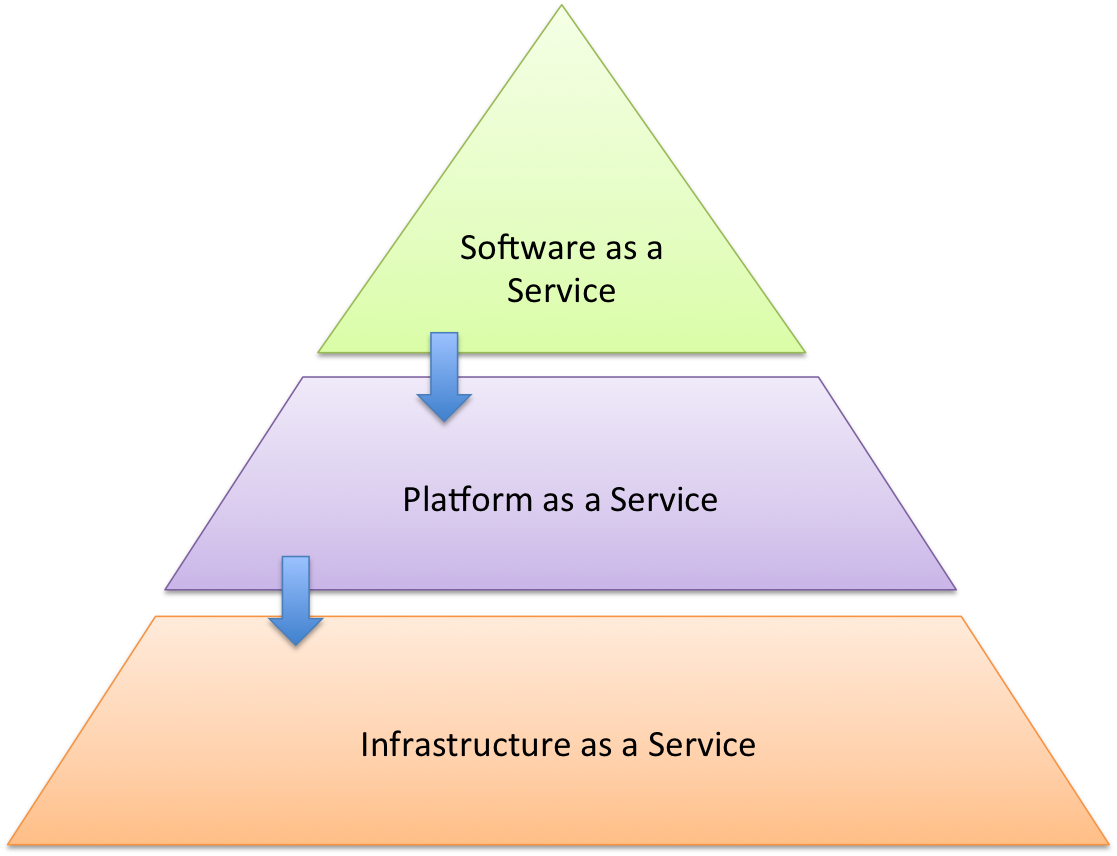
\includegraphics[width=.85\linewidth]{gfx/ipsaas}}
        \caption[The Cloud Computing Stack]{The Cloud Computing Stack}\label{fig:ipsaas}
    \end{center}
\end{figure}

For our purpose, the most important layer is the \ac{SaaS} layer. We want to connect to a cloud application that will provide us with the latest information and status of an already stablished service and allow us to interact with this information.

\section{Significance for Businesses}
Cloud technology is changing the way a lot of companies do business. Now, instead of expending thousands of dollars on server equipment and fiber networks, they can build their infrastructure on the cloud and scale the size of said infrastructure as needed. \cite{williams:2012}

Before the cloud became easily available, companies had to include more space and resources in their infrastructures than actually needed, in order to be able to handle unexpected growth periods.

Knowing how to get this balance right can be very tricky, though. If you include too little overhead and your service grows rapidly, the growth can overwhelm the service and stop it from becoming even greater. But if you plan for a lot of growth and invest a lot of money in extra infrastructure and the service never really takes off, the extra money spent on servers and bandwidth can bankrupt a small company.

This is all a thing of the past, thanks to scalability and high availability of cloud infrastructures. Using cloud technology to build your infrastructure will actually save you money, so a lot of companies are ditching their local infrastructure and upgrading to cloud technology.

This growth in the market has seen an increase in companies offering cloud infrastructure for rent. One of the biggest providers of \ac{IaaS} is Amazon, an online retailer. The fact that an online retailer has a bigger market share\footnote{\url{http://arstechnica.com/information-technology/2013/03/vmware-targets-rival-bookseller-amazon-with-its-own-public-cloud/}} in \ac{IaaS} than tech giants such as Microsoft and VMware, has baffled the industry and was the moving force behind the continuous investment these companies have made in the past year in order to offer the same kind of service and regain all the market they lost.\footnote{\url{http://arstechnica.com/information-technology/2013/08/amazon-and-microsoft-beware-vmware-cloud-is-more-ambitious-than-we-thought/}} 

\section{Influence of the Cloud in Mobile Applications}
The Cloud has had a big impact and influence on how mobile applications have evolved and changed over the past few years. Before the introduction of the Cloud we know today, mobile applications were fairly simple and often focused on productivity and personal organization. The first \ac{PDA} devices did just that. They came with a set of applications developed by the manufacturer and the user could not change the installed applications or add new ones. 

With the dawn of the mobile internet a new wave devices came that were capable of more that just productivity apps. The first applications to be connected to external services were E-Mail and Calendar. This choices were pretty obvious, since they rely on external and up-to-date data.

After mobile internet became faster and more ubiquitous, a new breed of applications started to emerge, applications that relied more and more on data retrieved from remote sources.

This has been the influence of the Cloud on mobile applications. Nowadays it is really hard to find a piece of mobile software that doesn't rely on or offer some kind of Cloud connectivity.  

The many aspects of the cloud, like ease of access, availability, ease of development and low entry cost have changed the mobile landscape and shaped it into what we all use now. Thanks to these technologies, mobile computing is going to continue to evolve and change for the better.





    





